\title{PartyMixer – Cocktails für zu Hause}
\team{%
    Kim Schenk,
    Robin Aebi}

\client{Kim Schenk,
		Robin Aebi}

\projtype{P6}

\coaches{%
	Pascal Schleuniger}

\fssummary{
Bei einer gelungenen Party darf eines auf keinen Fall fehlen, die Getränke. Diese sicherzustellen ist jedoch meistens mit viel Aufräumarbeit und Selbstaufwand verbunden. Genau da kommt der PartyMixer ins Spiel. Mit dem PartyMixer können sich die Gäste selbstständig die gewünschten Cocktails erstellen lassen und dies ganz ohne Chaos oder verschüttete Getränke.
}

\fsgraphics{
    \centering
\bigskip
\noindent
\begin{minipage}[t]{.4\textwidth}
\raggedright
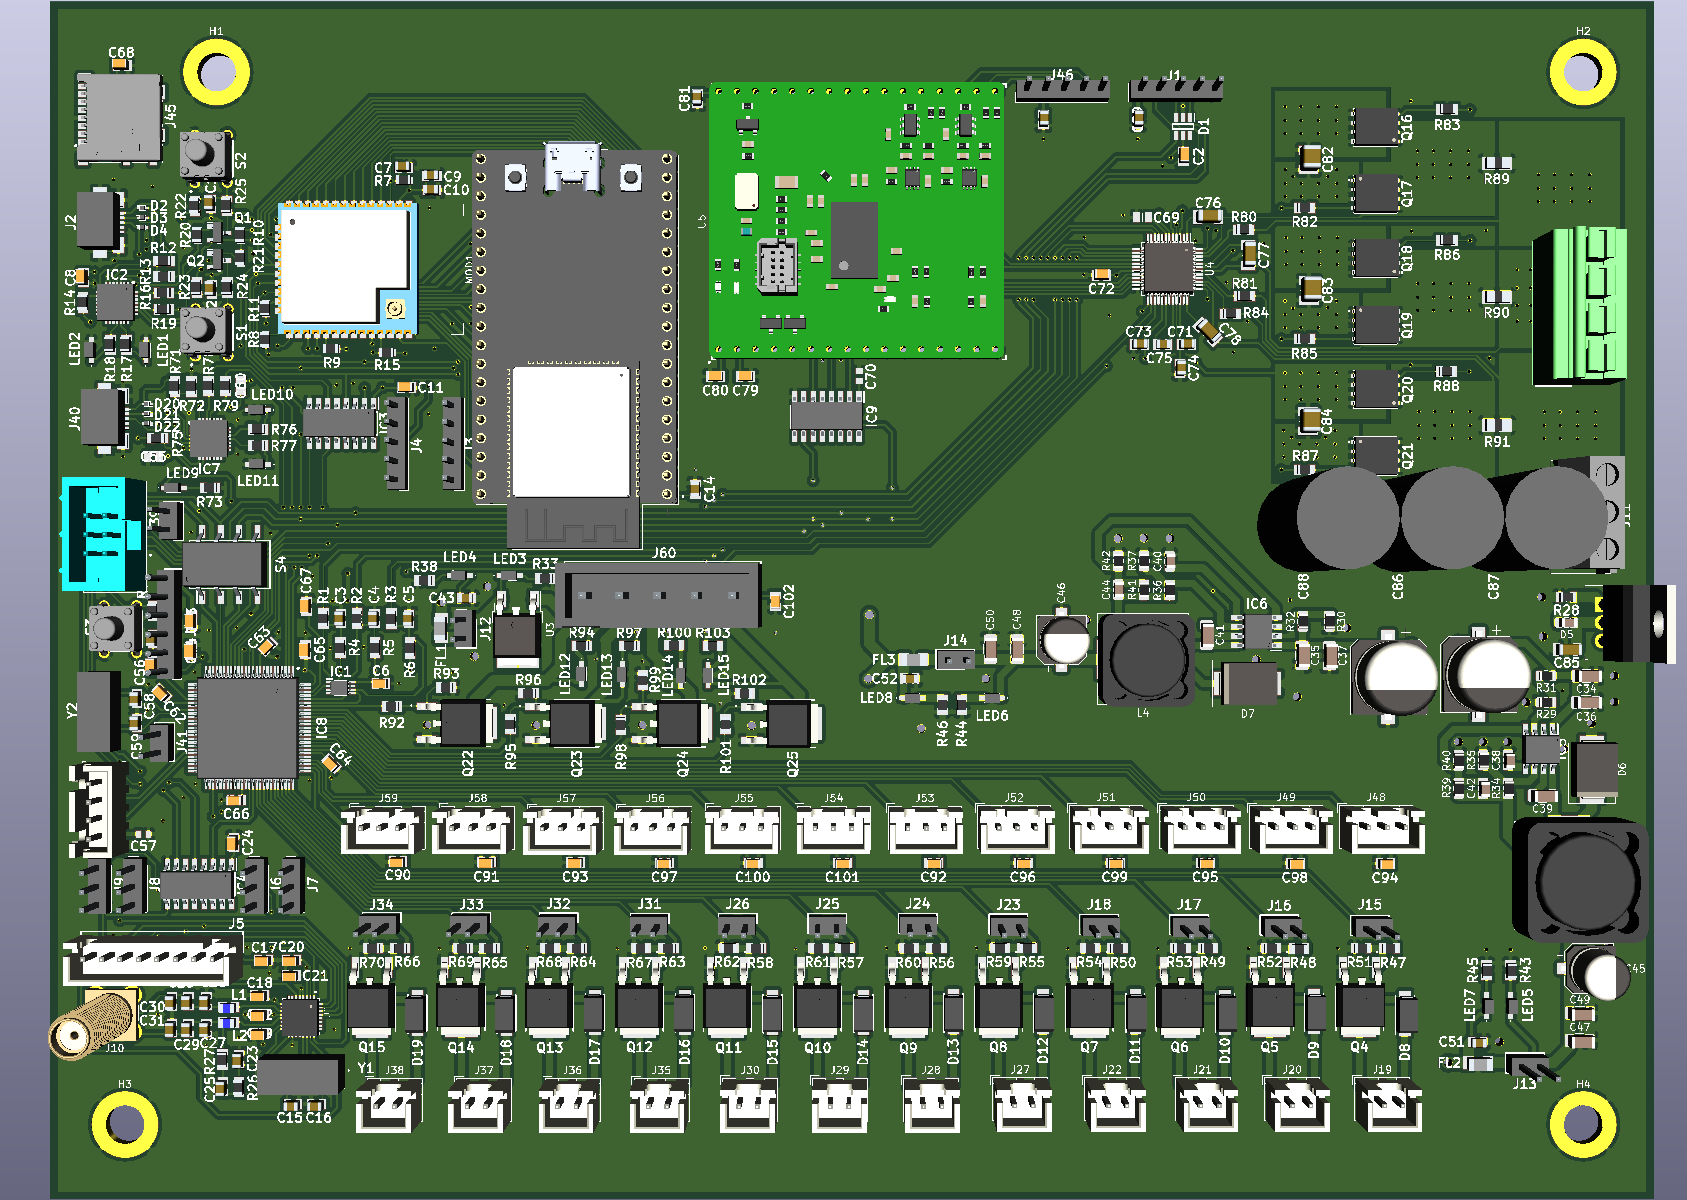
\includegraphics[height = 50mm]{images/Print_3D}\\
\graphicscaption{Print 3D-Modell (Hardware)}
\end{minipage}
\hfill
\noindent
\begin{minipage}[t]{.5\textwidth}
\raggedright
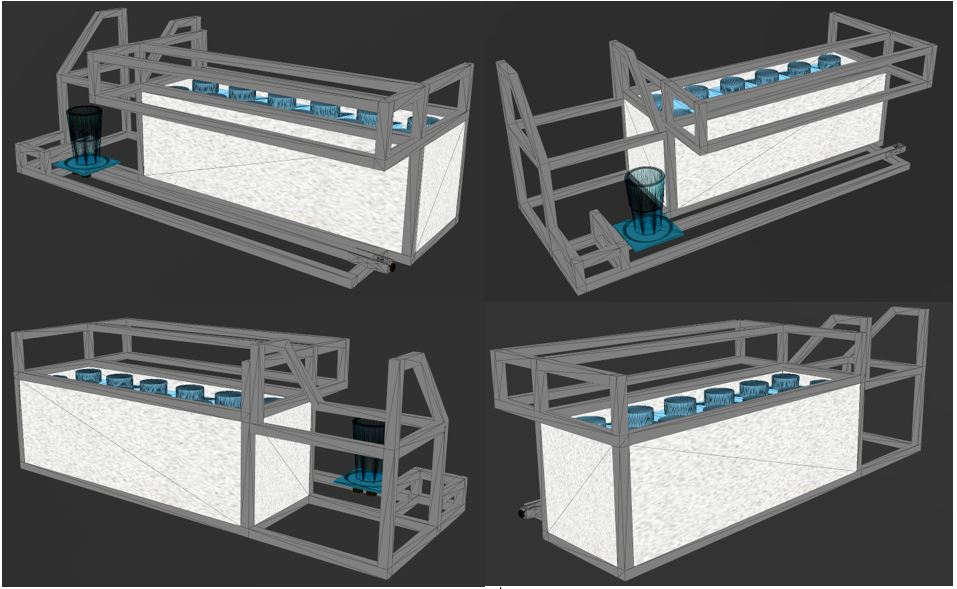
\includegraphics[height = 50mm]{images/3DModell}\\
\graphicscaption{Mechanik 3D-Modell (Mechanik)}
\end{minipage}
}

\fscontent{
    \section{Hardware}
	Die Hardware besteht aus einer Leiterplattine, worauf alle Komponenten für die gewünschten Funtkionen enthalten sind. Dazu gehören die Speisungen, der Mikrocontroller, die Motorengruppe, das WiFi-Modul, die Ansteuerung für die Pumpen und zugehörige Sensoren und die LED-Steuerung. Ausserdem wird ein externes RFID-Modul und Display verwendet.
    \section{Software}
	Der grösste Software-Teil gehört zum Mikrocontroller. Dieser steuert die Maschine an sich. Ein weiterer Software-Teil steckt in der Android-Applikation. Darin wird das User-Interface bereitgestellt und bei Berührungen des Displays Aktionen ausgelöst. Die ausgelösten Aktionen werden im WiFi-Modul verarbeitet. Das WiFi-Modul kommuniziert dann mit dem Mikrocontroller.
    \section{Mechanik}   
    Die Mechanik ist das Skelett der Maschine. Es trägt die angesteuerten Komponenten und stellt sicher, dass die Funktion der Maschine gewährleistet ist. Zur Mechanik gehören der Rahmen, der Getränkeschlitten, die Verleidung, die Unterbringung der Elektronik und die Kühlbox. Der LED-Streifen wird auch am Rahmen befestigt.
}

\infobox{Funktionen}{%
    \footnotesize
    \setlength\tabcolsep{2pt}
    \begin{tabular}{lp{100mm}lp{0mm}}
    \bfseries Cocktails  		&                         			& 	  &\\
    Cocktails können erstellt und bearbeitet werden. & hüü& & \\
    Die Position und Art der Zutaten ist frei wählbar. & & & \\
	Automatische Listenerstellung anhand der Zutaten. & & & \\
	\bfseries RFID & & & \\
	Cocktail kann einem Tag zugeordnet werden. & & & \\
	\bfseries Reinigung & & & \\
	Ein begleiteter Reinigungsmodus ist vorhanden. & & & \\
	
    \end{tabular}
}
